\section{Four-mark tests after exploration}\label{sec:slits}

Proposition~\ref{prop:polygon-comparison} concerns a fixed polygon.  The
conditional law seen by an exploration lives instead in a domain whose
boundary contains the entire past of the curve.  We now extend the
four-mark test to these remaining domains.  The main geometric step is
to place the relevant part of such a domain in a compact portion of a
covering surface.  A polygon in that surface still uses the original
square grid, so Proposition~\ref{prop:polygon-comparison} applies to it.

Throughout this Section we fix the deterministic subsequence and the
environment supplied by Lemma~\ref{lem:quenched-diagonal}.  In particular,
the fixed polygon limits hold simultaneously for the countable stock
of rational polygons on finitely many square-grid charts, for both
colors.  All probabilities below are quenched.  Limits of probabilities
are taken along this subsequence; a geometric radius is fixed before
the mesh tends to zero.

We use the simple drawings of Lemma~\ref{lem:compatible-drawing}.  A
\emph{history} is a prefix stopped by a rule that reveals only the
switches encountered by the strand.  Its remaining domain is the
slit disk $U_n$, viewed with its prime-end boundary.  Under separate
primal closure, the two primal boundary intervals are wired separately;
we call them the \emph{electrodes}.  An actual connection between them
uses open edges, together with the identifications within each
electrode.  A \emph{possible connection} means a connection after all
unrevealed edges of the tested color have been allowed, before any
jump along an external wire.  Known bank edges have the physical
accesses described in Lemma~\ref{lem:compatible-drawing}.

\begin{proposition}[Four-mark test in a remaining domain]
\label{prop:moving-test}
Consider the four-change open-cap law and any sequence of
switch-revealing stopping rules before completion of its strand.
Let $A_n$ be events determined by the stopped history.  Suppose that,
on $A_n$, there are basepoints $z_n$ and constants $r_0,\alpha_0>0$,
independent of $n$ and of the history, such that
\begin{enumerate}
\item $B(z_n,r_0)\subset U_n$;
\item in the conformal disk chart normalized at $z_n$, the four
  current prime-end marks, including the tip, have pairwise distance
  at least $\alpha_0$ on the unit circle.
\end{enumerate}
Assume also that the stopped prefixes form a tight family in the
oriented-curve topology, as in Proposition~\ref{prop:curve-tightness}.
Write $\mathcal F_n$ for the stopped information, $E_{\mathrm P}$ for
the primal pairing, and $\chi_{U_n}$ for the ordered cross-ratio of
the four current marks.  Then, for every $t>0$,
\begin{equation}\label{eq:slits-moving-test}
 \P_{\mathrm{open}}\left(
 A_n\cap\left\{
 \left|\P_{\mathrm{open}}(E_{\mathrm P}\mid\mathcal F_n)
             -f(\chi_{U_n})\right|>t\right\}\right)\longrightarrow0.
\end{equation}
The basepoints may be selected from the history.  The original domains
lie in a fixed bounded set, so every deterministic sequence of these
basepoints has a convergent subsequence.
\end{proposition}

The function $f$ is the open-cap function of
Proposition~\ref{prop:pure-four-mark}.  Under separate closure the
corresponding crossing function is
\begin{equation}\label{eq:slits-odds}
 g(\chi)=T(f(\chi)),\qquad
 T(p)=\frac{p}{p+\sqrt2(1-p)}.
\end{equation}
It will suffice to prove an upper bound by $g(\chi_{U_n})$ for the
conditional primal crossing probability.  The identical upper bound
for the dual crossing, together with
$f(1-\chi)=1-f(\chi)$ and the exact conditional change of closure,
will give both sides of \eqref{eq:slits-moving-test}.

\subsection{Physical access and the cost of deleting small balls}

The first two lemmas isolate the probabilistic part of the comparison.
They are the chart and deletion arguments of
\cite[Section ``Alternating tests after exploration'']{C}, with the
one-arm input replaced by Lemma~\ref{lem:full-grid-arm}.  We give their
proofs to specify precisely which boundary identifications are allowed.

Map $U_n$ to
\[
 R_n=(0,1)\times(0,h_n)
\]
so that the electrodes are the vertical sides, and let $u_n$ denote
the first coordinate.  The assumptions of
Proposition~\ref{prop:moving-test} keep $h_n$ in a compact subinterval
of $(0,\infty)$.

\begin{lemma}[Small physical paths have small chart oscillation]
\label{lem:slits-chart}
Under the base-disk and mark-separation assumptions above, there is a
common modulus $\omega(r)\downarrow0$ such that the oscillation of
$u_n$ on any connected path in $U_n$ of physical diameter at most $r$
is at most $\omega(r)$.  The statement includes prime-end accesses by
interior approximation.

Consequently, for every $\beta>0$, a possible connection starting in
\begin{equation}\label{eq:slits-wide-band}
 B_n(\beta)=\{\beta\leq u_n\leq1-\beta\}
\end{equation}
must travel a fixed positive physical distance before reaching an
electrode or a known open bank edge of the tested color, for all
sufficiently small meshes.  The distance is uniform in the history.
\end{lemma}

\begin{proof}
Choose a disk $O$ containing all physical domains with a fixed margin.
For a small ball away from $B(z_n,r_0/2)$, the probability that Brownian
motion from $z_n$ hits that ball before leaving $O$ tends uniformly to
zero with its radius.  For example, the logarithmic harmonic function
in an enclosing annulus gives a bound of order
$1/|\log r|$.  Killing earlier on leaving $U_n$ only decreases this
probability.

In the normalized unit disk, a connected set of diameter at least
$a>0$ has hitting probability from the origin bounded below by a
positive number depending only on $a$.  This is the crosscut form of
the Beurling estimate: a connected set joining two separated small
sectors is either met before exit or separates a boundary interval
of uniformly positive harmonic measure from the origin.  The estimate
also applies to connected sets close to the circle; the set itself,
rather than its boundary projection, lies in the disk.  Conformal
invariance therefore implies that a small physical path away from
the basepoint has small diameter in the disk chart.  Near the basepoint
the same conclusion follows from interior distortion on the fixed
base disk.  The maps from the disk to $R_n$ form a compact family on
the closed disk because the four angles remain separated.  This
proves the asserted modulus for $u_n$.

Every electrode attachment and every known open bank edge has an
access to $u_n=0$ or $u_n=1$ within $O(\delta_n)$, by
Lemma~\ref{lem:compatible-drawing}.  A short possible connection
from $B_n(\beta)$ to such an attachment would, after adding this
access, have chart oscillation at least $\beta$ and physical diameter
tending to zero.  Choose the physical distance so that its modulus
is smaller than $\beta/2$, and then absorb the tile error by taking
$n$ large.  This also shows that the two electrodes have not already
met along the revealed bank under the stated localization.
\end{proof}

\begin{lemma}[Deletion in a central band]\label{lem:slits-deletion}
Fix a history and use separate closure for the tested color.  Delete
a set $S$ of unrevealed edges.  The change in the probability of an
actual electrode-to-electrode connection is at most the original
conditional probability that an endpoint of an edge in $S$ has an
actual connection to an electrode, allowing one edge of $S$ as an
initial test step.

If the deleted incidences lie in $B_n(\beta)$ and in a union of $m$
balls of radius $r$, where $m$ is fixed, this cost tends to zero
uniformly in their centers and in the histories, in the order
\[
 \lim_{r\downarrow0}\limsup_{n\to\infty}.
\]
The same conclusion holds with a fixed number of nested bands and
slightly enlarged balls.
\end{lemma}

\begin{proof}
Couple the original law and the law with the edges in $S$ closed
monotonically.  Explore, in the stronger configuration, the actual
clusters from the deletion endpoints, revealing their incident edges
in both configurations.  FK partition monotonicity remains valid at
each step.  Once these clusters are enclosed by their closed edge
cuts, the conditional laws outside agree and may be coupled
identically.  If no explored cluster reaches an electrode, the
crossing decision is the same.  Known connections along a bank count
as electrode access in this argument.

For the second assertion choose an outer radius $R_\beta>0$ using
Lemma~\ref{lem:slits-chart}.  Every component of possible edges in
a ball of radius $R_\beta$ that meets the deleted central incidences
has no accessible wire or known open attachment there.  All its
remaining boundary identifications arise at the rim of the ball.
Project this graph to the physical grid, fill missing edges, identify
any copies of a physical vertex, and wire the rim.  These operations
increase the induced FK partition and dominate its actual arm event.
Cropping the annulus by a few tile widths accommodates the drawing
and the possible initial test step.  Lemma~\ref{lem:full-grid-arm}
bounds the resulting probability of an arm from radius $r$ to
$R_\beta$ by a quantity tending to zero in the asserted order.  A
union bound over the fixed $m$ balls completes the proof.
\end{proof}

\subsection{Fibers that become crosscuts of a cover}

We next construct a comparison domain without regularizing the slit
boundary itself.  The argument is deterministic.  Consider a sequence
of localized histories whose prefixes converge after increasing
reparametrizations.  The initial boundary curves converge as well.
After passage to a subsequence, the basepoints converge to $z$, the
remaining domains have pointed kernel $U$, their boundaries have a
Hausdorff limit, and the four normalized boundary angles converge.
Here $U$ means the component containing $z$.  The normalized maps
from the disk converge on compact subsets, as do the inverse
rectangle parametrizations, which we denote by
$F_n:R_n\to U_n$.  Every point of $\partial U$ is approached by
complements of $U_n$.  These uses of normalized kernel convergence
and prime-end parametrization are the usual conformal mapping facts; see
\cite{Pommerenke}.

Fix a small trimming parameter $a_*>0$, and then choose
$0<\beta<a_*/20$.  We shall compare the original crossing with a
test between the levels $a_*$ and $1-a_*$.  To control the coordinates
of every possible path between these levels, choose ordered disjoint
abscissa bins, each of width at most $\lambda$ and with every
intervening gap at most $\lambda$, where $\lambda\ll\beta$.
Their convex hull contains
$[2\beta,1-2\beta]$.  Include one bin in $(2\beta,3\beta)$ and one
in $(1-3\beta,1-2\beta)$; the fibers chosen in these two bins will
be called the \emph{anchor fibers}.  These are distinguished members
of the family, not necessarily its extreme fibers; the other bins
may extend beyond them toward the electrodes.

\begin{lemma}[Choice of fibers]\label{lem:slits-fibers}
For every prescribed physical tail radius $r>0$, one can choose a
simple top-to-bottom fiber in each bin, and pass to a subsequence,
with the following properties.
\begin{enumerate}
\item Each fiber stays in its bin in rectangle coordinates.  Apart
  from a top and a bottom tail, it converges inside a compact subset
  of $U$.  Each tail is contained in a physical ball of radius $r$.
\item All physical endpoints of all the fibers have distinct limits.
\item The fibers are mutually disjoint and ordered by their bins.
\end{enumerate}
The omitted top and bottom portions may have fixed, sufficiently
small fractions of the rectangle height.  The two half-fibers may
use different abscissas within the same bin.
\end{lemma}

\begin{proof}
Let $I$ be one bin and let $J$ be a short interval adjacent to the
top or bottom of $R_n$.  By Cauchy--Schwarz,
\begin{equation}\label{eq:slits-length-area}
 \int_I \operatorname{length}
       \bigl(F_n(\{x\}\times J)\bigr)\,dx
 \leq (|I||J|)^{1/2}
       \left(\int_{I\times J}|F_n'(w)|^2\,dA(w)\right)^{1/2}.
\end{equation}
The last integral is at most the area of the common physical
enclosing disk.  By making the height fraction sufficiently small,
the set of levels with tail length exceeding $r$ occupies an
arbitrarily small fraction of $I$.

We can simultaneously separate the endpoints.  On the compact
portions of the horizontal rectangle sides containing the bins,
harmonic measure from the basepoint is uniformly comparable to
abscissa length.  An endpoint in a small physical ball contributes
at most the Brownian probability of reaching that ball before
leaving the enclosing disk.  This tends uniformly to zero as the
ball shrinks, by the logarithmic estimate used in
Lemma~\ref{lem:slits-chart}.  Choose the endpoints successively,
excluding fixed small balls around the endpoints already chosen.
There are only finitely many choices, and these exclusions together
with the length exclusions occupy less than the bin.  A positive
separation can therefore be retained before taking a subsequence.

Choose the top and bottom levels independently, then join them by
an interpolation inside the middle of the same bin.  Interior
convergence of $F_n$ gives convergence of the retained cores after
a further subsequence.  Different bins are disjoint, so the resulting
fibers are disjoint and ordered.  Endpoints can be chosen away from
the finitely many tile corners and exceptional prime accesses.
\end{proof}

Fix an enclosing disk $O$ with a positive margin around all physical
domains.  We enlarge the domain by removing only finitely many
physical points from $O$ and passing to a universal cover.  Include every selected
fiber endpoint among these punctures.  Add finitely many points of
$O\setminus U_n$ whose distinct limits sample $\partial U$ as finely
as required.  Write the resulting set as $P_n$ and its set of
distinct limits as $P$.  Let
\[
 \pi_n:\widetilde O_n\longrightarrow O\setminus P_n
\]
be the universal cover, with a chosen lift of $z_n$.  Its disk
uniformization is normalized by sending $0$ to this lift and making
the derivative of the projection positive at $0$.  Since $U_n$ is
simply connected, its inclusion has a unique lift
\[
 \iota_n:U_n\longrightarrow\widetilde O_n
\]
through the chosen basepoint.  This lift is injective, because
$\pi_n\circ\iota_n$ is the inclusion.  The surface has the ordinary
physical coordinate in every sufficiently small chart; there are
no branch points.

\begin{lemma}[Cover charts and strip trapping]\label{lem:slits-cover}
By choosing the finite boundary sample sufficiently fine, the disk
charts of $\widetilde O_n$ on the retained fiber cores and any fixed
compact access paths in $U$ can be made arbitrarily close to those
of $U_n$, for all sufficiently large $n$.

Give $\widetilde O_n$ rectangle coordinates using the same four disk
angles as for $U_n$, and denote their horizontal coordinate by
$v_n$.  After the tail radius and chart error have been chosen
sufficiently small relative to the bin spacing, each lifted fiber
is a crosscut of the cover rectangle, joining its horizontal sides
and lying in the corresponding abscissa bin with an arbitrarily
small enlargement.  Consequently
\begin{equation}\label{eq:slits-chart-matching}
 |v_n\circ\iota_n-u_n|\leq C\lambda
\end{equation}
between the two extreme fibers.  If $\Gamma_n^-$ and $\Gamma_n^+$
are the first and last fibers, respectively, then
\begin{align*}
 v_n(\iota_n(w))&\leq
     \sup_{\iota_n(\Gamma_n^-)}v_n
       &&\text{on the left electrode side of }\Gamma_n^-,\\
 v_n(\iota_n(w))&\geq
     \inf_{\iota_n(\Gamma_n^+)}v_n
       &&\text{on the right electrode side of }\Gamma_n^+.
\end{align*}
In particular, the enlarged extreme bins bound these coordinates
strictly outside the future test cuts at $a_*$ and $1-a_*$.
\end{lemma}

\begin{proof}
First consider increasingly fine finite samples of $\partial U$.
The normalized projections from the unit disk to the punctured
domains form a bounded normal family.  Their derivative at $0$ is
bounded below by the radius of the common base disk: that disk lifts
to the cover, and Schwarz's lemma gives the derivative comparison.
Any subsequential limit is therefore nonconstant.  Hurwitz's theorem
shows that it omits each point of the dense boundary sample.  Its
image is consequently contained in $U$, the component at $z$.

Conversely, every simply connected domain compactly contained in
$U$ and containing $z$ lifts into all the covers under consideration
once $n$ is large.  The same derivative comparison bounds the
projection derivative below by the conformal radius of that domain.
Exhausting $U$ and then applying Schwarz's lemma to the limit map
into $U$ shows equality with the conformal radius of $U$.  Thus the
limit is precisely the normalized Riemann map onto $U$.  This proves
the asserted approximation on compact sets and along their access
paths.  The order is to fix the desired compact accuracy, choose
a finite puncture list, and only then let $n$ tend to infinity.

For a fixed list with distinct limiting punctures, the charts of
the covers converge under continuation in physical coordinates.
One direct verification is to move the finitely many punctures by
diffeomorphisms supported in disjoint small neighborhoods, fixing
the base disk and the outer boundary, with dilatations tending to
one.  Their lifts, in normalized disk coordinates, converge to the
identity.  On every compact set away from the punctures this
identifies the limiting cover charts and preserves continuation
along any fixed finite collection of paths.

Consider now a fiber tail.  Its projection lies in a ball of radius
$r$ away from the basepoint.  Brownian motion on the cover, projected
to $O$, gives the same upper bound for hitting this tail as for
hitting its physical ball before exit from $O$.  The connected-set
estimate in the unit disk used in Lemma~\ref{lem:slits-chart} thus
makes its diameter small in the cover's disk coordinate.  The
disk-to-rectangle maps form a compact family on the closure, so
its rectangle diameter is small as well.  Apply this observation
to successively shorter tails approaching the endpoint.  The lift
has a continuous endpoint in the closed uniformizing disk.  That
endpoint cannot be interior: its projection tends to a puncture.
It is therefore an ideal boundary point of the cover.

On the retained core, both charts are close to the limiting chart
of $U$.  Taking the omitted height fractions small locates the top
and bottom endpoints near the corresponding horizontal sides,
away from their corners.  The lifted fiber is consequently a
crosscut joining those sides.  Its entire $v_n$-range lies in its
bin with a small enlargement.  These crosscuts are disjoint because
$\iota_n$ is injective, and their order is the order seen on the
common compact cores.

Each crosscut separates the whole cover disk into two components.
The two components of $U_n$ cut by its original fiber lift to the
corresponding sides: each is connected, and the side is determined
on an interior core.  A point between consecutive fibers is
therefore trapped between their lifted crosscuts.  Both its $u_n$
and $v_n$ coordinates lie between the adjacent bins, up to the
chosen errors.  This proves \eqref{eq:slits-chart-matching}.  The
same separation argument outside the two extreme fibers gives the
one-sided bounds.  In particular, the conclusion is global in the
lifted domain; compact convergence alone would not give it.
\end{proof}

\subsection{Keeping the relevant graph in finitely many charts}

The cover has infinitely many sheets.  To apply a fixed polygon test,
we must contain every relevant central incidence in one compact
portion of it.  A bounded physical region and positive puncture
clearance alone would allow arbitrarily many windings around a
puncture.  We will instead construct one access path to each relevant
point with a bounded number of fixed-size displacements; clearance
then bounds the number of chart continuations needed to lift it.
We first delete edges near the finitely many punctures.
The cost of these deletions is controlled by
Lemma~\ref{lem:slits-deletion}; tightness of the histories will control
the number of sheets that remain accessible.

Two different deletions serve this construction.  Removing the
anchor tails forces a central path toward an electrode to cross
a retained anchor core.  The smaller puncture neighborhoods give
the clearance needed to control the lift of that path and its
continuation from the core to the basepoint.  In the whole band
$B_n(\beta)$ make the following deletions:
\begin{enumerate}
\item delete uncertain edges in slightly enlarged balls containing
  the four tails of the two anchor fibers;
\item delete uncertain edges in small balls about every puncture
  of $P_n$.
\end{enumerate}
The tail radius was chosen during Lemma~\ref{lem:slits-fibers}.
Choose the second set of radii only after the finite puncture list
has been fixed.  They may be made small enough that the retained
anchor cores and fixed compact paths joining those cores to the
basepoint have positive clearance from this second set of balls.
No such clearance from the larger tail balls is required of these
auxiliary paths.  All radii are positive and fixed before the mesh
limit.  Lemma~\ref{lem:slits-deletion} makes the total crossing cost
arbitrarily small, first for the four tail balls and then for the
fixed finite number of puncture balls.

In the resulting graph, call an edge or vertex a \emph{candidate}
if its component of possible edges can reach an electrode.  Components
without possible electrode access can be discarded: they cannot
contribute to a crossing or attach to a component that can.

\begin{lemma}[Compact containment of central candidates]
\label{lem:slits-compact-candidates}
After these deletions, all candidate incidences in
$B_n(5\beta)$ lift into a fixed compact part of the limiting cover
charts, for all sufficiently large $n$.
\end{lemma}

\begin{proof}
Start from a central candidate and follow a possible connection
toward an electrode until its first exit from $B_n(\beta)$.
Lemma~\ref{lem:slits-chart} excludes a wire jump before this exit.
The path crosses the anchor fiber on that side.  Up to this crossing
it lies in the band where the puncture-ball edges were deleted, so
it stays away from the punctures.  Its crossing of the anchor cannot
be in a deleted tail.  Following the retained anchor core and then
one of its fixed compact access paths joins the candidate to the
basepoint while still avoiding the smaller puncture balls.  Physical
accesses at vertices can be shifted slightly into $U_n$, retaining
this clearance; tile errors are smaller than every fixed margin.

We show that all points accessible in this way have bounded sheet
indices.  Trim $U_n$ by mutually disjoint disks centered at $P_n$,
with slightly smaller positive radii than the second deletion radii,
and let $T_n$ be the component containing $z_n$.  The preceding paths
put all the central candidates in $T_n$, or in its boundary accesses.
The trimming circles can be chosen in general position, so that
they meet the finite polygonal slit drawing transversely in finitely
many points.

The prime boundary of $T_n$ consists of inherited portions of the
prime boundary of $U_n$, in their original cyclic order, interleaved
with arcs of the trimming circles.  To verify this description, note
that each puncture disk reaches the complement of $U_n$.  A whole
circle surrounding its center cannot lie in the simply connected
domain $U_n$.  Each portion of a trimming circle inside $U_n$ is
therefore a crosscut in the prime-end disk: its two physical
endpoints may coincide on opposite slit banks, but its endpoint
accesses are distinct.  The crosscuts from the disjoint trimming
circles are disjoint, and successive crosscut separation gives the
asserted boundary description of each remaining component.  The
two banks of the slit are counted separately in this description.

The inserted circle arcs have uniformly bounded total length: on
each circle their interiors are disjoint.  The inherited boundary
has a uniform bound on the number of successive oscillations of
every fixed positive size.  Indeed, it consists of the original
boundary traversal and two traversals of the prefix; the original
boundaries converge uniformly and the prefixes belong to a compact
family of curves.  The same oscillation bound holds for the trimmed
boundary.  More explicitly, subdivide the original parametrization
into a bounded number of pieces of diameter less than a prescribed
small fraction of the oscillation scale.  Inherited arcs occur in
that order.  Inserted arcs whose endpoints lie in one such piece
can make a substantial additional excursion only if their length
exceeds a fixed fraction of the scale.  Their number is bounded by
the total circle length.  Arcs crossing subdivision points account
for only a bounded number of further changes.

It remains to turn this boundary control into control of an access
path.  Join a point of $T_n$ and $z_n$ by straight segments to their
first boundary hits, and connect the two resulting prime accesses
along the trimmed boundary.  The straight segments have bounded
length.  The intervening boundary path has the oscillation bound
just established.  Polygonal prime-boundary paths admit arbitrarily
close interior approximations with those accesses, including on
the two sides of a slit.  Thus one obtains an interior path from
$z_n$ to the point with uniformly bounded oscillation count at a
fixed scale smaller than its clearance from every puncture.  An
additional arbitrarily short access segment handles a boundary
incidence.

Cover the common compact physical region away from the punctures
by finitely many ordinary chart disks, smaller than this clearance.
Subdivide the access path whenever its diameter reaches a still
smaller fixed scale.  There are boundedly many pieces, and each
lies in one of these ordinary disks.  Its lift is obtained by a
bounded number of continuations among a finite list of charts,
so it lies in a compact part of the universal cover.  The same
compact chart bound works for the varying punctures by
Lemma~\ref{lem:slits-cover}.  Only one controlled access path is
needed for each point: any other path in $U_n$ reaches the same
lift because $\iota_n$ is single-valued.  This proves the lemma.
\end{proof}

\begin{figure}[t]
\centering
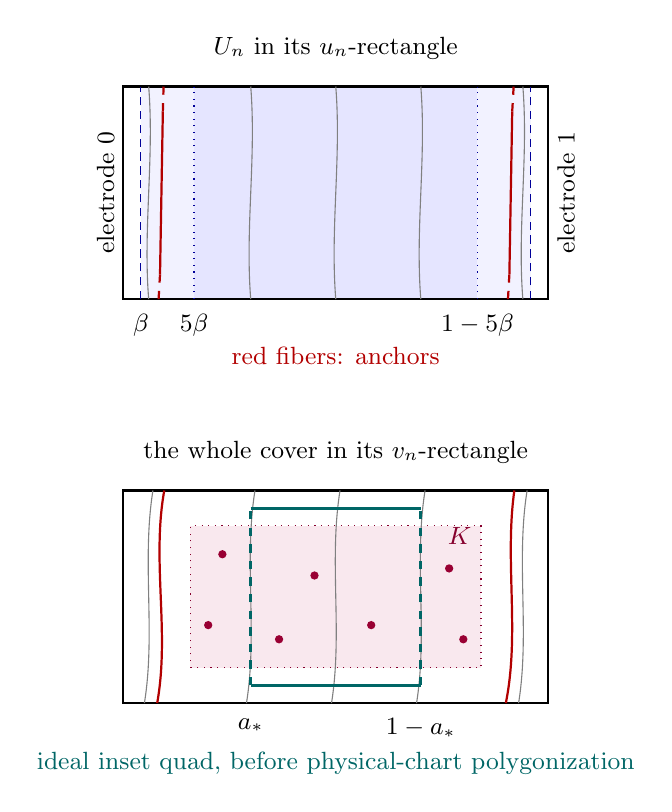
\begin{tikzpicture}[x=0.9cm,y=0.9cm,>=stealth,
  every node/.style={font=\small}]
\begin{scope}
 \fill[blue!5] (0.25,0) rectangle (5.75,3);
 \fill[blue!10] (1,0) rectangle (5,3);
 \draw[thick] (0,0) rectangle (6,3);
 \draw[blue!60!black,densely dashed] (0.25,0)--(0.25,3);
 \draw[blue!60!black,densely dashed] (5.75,0)--(5.75,3);
 \draw[blue!60!black,dotted] (1,0)--(1,3);
 \draw[blue!60!black,dotted] (5,0)--(5,3);
 \foreach \x in {0.36,1.8,3,4.2,5.64} {
  \draw[gray] (\x,0) .. controls (\x-0.08,1) and (\x+0.08,2) .. (\x,3);
 }
 \draw[red!70!black,thick] (0.52,0.35)--(0.56,2.65);
 \draw[red!70!black,thick] (5.45,0.35)--(5.49,2.65);
 \draw[red!70!black,thick,dashed] (0.50,0)--(0.52,0.35);
 \draw[red!70!black,thick,dashed] (0.56,2.65)--(0.57,3);
 \draw[red!70!black,thick,dashed] (5.43,0)--(5.45,0.35);
 \draw[red!70!black,thick,dashed] (5.49,2.65)--(5.51,3);
 \node[above] at (3,3.25) {$U_n$ in its $u_n$-rectangle};
 \node[rotate=90] at (-0.25,1.5) {electrode $0$};
 \node[rotate=90] at (6.25,1.5) {electrode $1$};
 \node[below] at (0.25,-0.08) {$\beta$};
 \node[below] at (1,-0.08) {$5\beta$};
 \node[below] at (5,-0.08) {$1-5\beta$};
 \node[red!70!black] at (3,-0.8) {red fibers: anchors};
\end{scope}
\begin{scope}[shift={(0,-5.7)}]
 \draw[thick] (0,0) rectangle (6,3);
 \fill[purple!9] (0.95,0.5) rectangle (5.05,2.5);
 \draw[purple!70!black,dotted] (0.95,0.5) rectangle (5.05,2.5);
 \draw[red!70!black,thick] (0.48,0)
  .. controls (0.66,1) and (0.40,2) .. (0.58,3);
 \draw[red!70!black,thick] (5.40,0)
  .. controls (5.60,1) and (5.38,2) .. (5.52,3);
 \foreach \x in {0.36,1.8,3,4.2,5.64} {
  \draw[gray] (\x-0.06,0)
   .. controls (\x+0.1,1) and (\x-0.1,2) .. (\x+0.06,3);
 }
 \draw[teal!80!black,very thick] (1.8,0.25)--(4.2,0.25);
 \draw[teal!80!black,very thick] (1.8,2.75)--(4.2,2.75);
 \draw[teal!80!black,very thick,dashed] (1.8,0.25)--(1.8,2.75);
 \draw[teal!80!black,very thick,dashed] (4.2,0.25)--(4.2,2.75);
 \foreach \x/\y in {1.2/1.1,1.4/2.1,2.2/0.9,2.7/1.8,3.5/1.1,4.6/1.9,4.8/0.9} {
  \fill[purple!80!black] (\x,\y) circle (1.5pt);
 }
 \node[above] at (3,3.25) {the whole cover in its $v_n$-rectangle};
 \node[below] at (1.8,-0.08) {$a_*$};
 \node[below] at (4.2,-0.08) {$1-a_*$};
 \node[purple!70!black,anchor=east] at (5.05,2.36) {$K$};
 \node[teal!80!black,align=center] at (3,-0.85)
  {ideal inset quad, before physical-chart polygonization};
\end{scope}
\end{tikzpicture}
\caption{Coordinate trapping and compact containment, schematically
and not to scale;
only a few of the finely spaced fibers are shown.
Fibers in separated bins become ordered crosscuts of the universal
cover; their coordinates agree up to the error in
\eqref{eq:slits-chart-matching}, not exactly.  Their separation
controls the coordinates throughout the lifted domain.  After the deletions, the central candidates lie in a
compact set $K$, shown inside a rectangular compact enclosure in the
lower panel.  The horizontal test sides can therefore be inset by
less than their distance from $K$.  Candidates may extend past both
vertical cuts; those exterior pieces may attach only to the wired
test electrodes.  The teal rectangle is the ideal inset quad; it
is subsequently approximated by a fixed orthogonal polygon in
physical-coordinate charts.  Dashed anchor ends in the upper panel indicate
the tails covered by deletion balls in physical coordinates.}
\label{fig:slits-cover}
\end{figure}

\subsection{A fixed polygon and its FK comparison}

We can now choose the polygon to which the fixed-domain theorem will
be applied.  In the limiting cover rectangle, cut at
$v=a_*$ and $v=1-a_*$.  Place the horizontal sides a small positive
distance inside the top and bottom.  By
Lemma~\ref{lem:slits-compact-candidates}, this distance can be chosen
so small that every central candidate lies strictly on the inner
side of both horizontal walls, with a positive margin.  The resulting
quad is relatively compact in the cover.  Figure~\ref{fig:slits-cover}
shows the distinction between this horizontal containment and the
two vertical cuts, across which candidate paths are allowed to pass.

Approximate the quad by a rational horizontal--vertical polygon
in physical-coordinate charts, with still smaller error and a compact
collar.  Such approximations can be constructed first by polygonal
curves, then by staircases in disjoint thin corridors, and finally
by joining the staircases in disjoint small vertex neighborhoods.
The marked points can be put in straight side interiors.  Uniform
Jordan convergence in a disk chart of the surface implies convergence
of the marked moduli.  Thus the approximation errors can be chosen
after all the preceding margins have been fixed.

\begin{lemma}[The comparison polygon is a fixed test]
\label{lem:slits-fixed-test}
The polygon just constructed may be chosen from the countable stock
in Lemma~\ref{lem:quenched-diagonal}.  For all sufficiently large $n$,
its rounded graph on the varying cover uses the same finite system
of physical-coordinate charts and the same incidence data.  Its
quenched crossing probability therefore converges to the pure
four-mark value for this fixed polygon.
\end{lemma}

\begin{proof}
A compact collared polygon away from the punctures is covered by
finitely many ordinary projection charts.  Choose rational rectangles
inside these charts, with overlaps large enough for the required
continuations.  Their gluings have identity projection transitions.
Subdividing further, the polygon and a collar can be specified by
finitely many rational rectangles or squares, their sheet labels,
and the incidence identifications on overlaps.  There are countably
many finite descriptions of this kind, including when projections
of different sheets overlap.

These finite chart continuations stay a positive distance from the
limiting punctures.  As the punctures move, the same projected paths
and neighborhoods avoid them, and their lift identifications agree
for all large $n$, by the finite-list continuity in
Lemma~\ref{lem:slits-cover}.  Thus both the physical polygon and its
square-grid rounding have fixed chart and incidence descriptions.
Copies of the same physical edge have the same disorder, exactly
as in Proposition~\ref{prop:polygon-comparison}; they are distinct
FK edges when they lie on different sheets.  The simultaneous
fixed-test limit on the chosen environment, followed by
Proposition~\ref{prop:pure-four-mark}, gives the assertion.
\end{proof}

The next comparison is between finite FK graphs, before any limit is
taken.  Let $H_n$ be the conditional graph after the deletions and
discard the components without possible electrode access.  Let
$Q_n$ be the rounded fixed test on the cover.  An edge is
\emph{shared} if it is a remaining central candidate edge of $H_n$
and its lift is an edge of $Q_n$.  We include all edges in the closure
of the rounded test, so an edge path leaving through a vertical
side has a vertex on the corresponding test electrode.

\begin{lemma}[Comparison on shared edges]\label{lem:slits-shared}
For sufficiently small geometric errors and sufficiently large $n$,
\begin{equation}\label{eq:slits-shared-comparison}
 \phi_{H_n}(\text{actual original-electrode crossing})
 \leq
 \phi_{Q_n}^{\mathrm{sep}}(\text{test-electrode crossing}),
\end{equation}
where $\phi_{H_n}$ is the conditional FK law and the two test
electrodes are wired separately in $\phi_{Q_n}^{\mathrm{sep}}$.
\end{lemma}

\begin{proof}
Take the central range for shared edges inside $B_n(5\beta)$,
allowing fixed smaller margins at its boundary.  Since
$\beta<a_*/20$, this range extends well past both vertical test
cuts.  The chart errors in
\eqref{eq:slits-chart-matching} and the polygonization error are
chosen much smaller than these margins.

There is no attachment from a shared edge to a nonshared original
piece through a horizontal test side.  Indeed, every possible
central attachment belongs to the compact candidate set, which
lies on the inner side of those walls with positive clearance.
A noncentral piece cannot enter there either: the global strip
trapping and its one-sided bounds put such pieces beyond the
corresponding vertical cut.  Consequently a nonshared original
piece can attach to the shared graph only along one of the two
test electrodes.

Nor can a nonshared piece connect the two electrodes to each other.
Between small neighborhoods of the vertical cuts there is a middle
strip in which every candidate edge is shared.  A possible path
from the left exterior group to the right must traverse that strip,
by \eqref{eq:slits-chart-matching}.  All identifications from known
banks and original wires belong to the separate left and right
groups: Lemma~\ref{lem:slits-chart} excludes a central access to
either wire and excludes an already known connection between them.

These statements remain valid when the drawing is matched to
physical lattice vertices.  Each uncertain switch supplies only
one random edge, by Lemma~\ref{lem:compatible-drawing}.  For a
primal-open switch, the primal bank follows the revealed ordinary
edge, attaching both endpoint vertex regions to that bank.  For a
primal-closed switch, the encountered turn cuts off only its visited
primal corner, where the bank stays at the same vertex.  The opposite,
unvisited corner retains a connected small neighborhood of its
incidences.  If that other turn is visited later, the same rule then
attaches its corner to the bank.  Thus every vertex whose required
identifications have been separated by the explored strand is
already bank-attached and is excluded from the central band by
Lemma~\ref{lem:slits-chart}.

The boundary construction retains all interior incidences of a
primal boundary vertex.  Exterior dual tabs are separate vertices
of the drawn graph.  Apart from the prescribed electrode-wire
identifications already handled above, distinct tabs require no
identification with one another, and the comparison does not merge
their different lifts.  If two such copies occupy the same ordinary
vertex in one lifted test chart, their merger in the test only
strengthens the local partition.  Interchanging the two colors
gives the same switch argument for a dual test.
Consequently all identifications required among the remaining
unbanked incidences have representatives in a common small vertex
neighborhood.  Away from the puncture balls these representatives
have a common local lift, identical to that of the ordinary grid
incidences.  No additional central identification can therefore join
different sheets or connect the two exterior groups around the shared strip.

Condition now on all nonshared original edges.  Their induced
partition on the shared graph identifies vertices only within
one test electrode or within the other.  It is therefore dominated
by the partition that wires each test electrode separately.
The weights on every shared edge are exactly those in $Q_n$.
Adding the remaining test edges and applying FK monotonicity gives
a stochastic upper comparison on the shared graph.  Finally, every
actual original crossing contains a shared-edge crossing between
the two test electrodes: take its traversal from the left exterior
group to the right, and use the absence of any nonshared bypass.
This event inclusion and the conditional stochastic comparison prove
\eqref{eq:slits-shared-comparison} after averaging the conditioned
edges.  The proof is unchanged for the dual grid and its actual odds.
\end{proof}

\subsection{Completion of the moving test and order of limits}

\begin{proof}[Proof of Proposition~\ref{prop:moving-test}]
Suppose that \eqref{eq:slits-moving-test} fails with a fixed positive
error and a fixed positive probability along a subsequence.
Tightness of the prefixes lets us restrict to a compact family of
curves while losing less than this probability.  In particular,
their numbers of successive displacements of every fixed size
have deterministic bounds on that family.  Select a deterministic
failing history at each remaining mesh.  The initial boundaries
already converge, so we may take the convergent-prefix, basepoint,
angle, and kernel subsequences used above.

It is enough to contradict failure of an upper crossing bound in
one of the two separate closures.  Indeed, if $p_n$ is the
conditional open-cap pairing probability, those crossing
probabilities are exactly $T(p_n)$ and $T(1-p_n)$, respectively,
by Lemma~\ref{lem:cap-change}.  The continuous increasing
map $T$ has a continuous inverse on $[0,1]$.  The two upper bounds
by $g(\chi_{U_n})=T(f(\chi_{U_n}))$ and
$g(1-\chi_{U_n})=T(1-f(\chi_{U_n}))$ therefore force
$p_n-f(\chi_{U_n})\to0$.

Fix an error tolerance.  Choose $a_*$ small, then $\beta<a_*/20$
and the fiber-bin precision $\lambda$ much smaller than $\beta$.
Choose the tail radius so that the four anchor-tail deletions have
small total cost and the lifted tails have sufficiently small chart
diameter.  Lemma~\ref{lem:slits-fibers} gives a fixed finite number
of fibers and their limiting endpoints.  Choose a fixed finite
puncture sample fine enough for Lemma~\ref{lem:slits-cover}.  Only
after that choice, take the puncture-ball radii small enough for
both the required core clearances and a small total deletion cost.
Lemma~\ref{lem:slits-compact-candidates} then gives one compact
part of the cover containing the surviving central candidates.
Choose the horizontal inset of the test smaller than the clearance
of this compact set, and finally choose the rational polygon with
strictly smaller approximation errors.

All these data are fixed before taking the mesh limit.  The
deletion bound and Lemmas~\ref{lem:slits-fixed-test}
and~\ref{lem:slits-shared} give
\[
 \limsup_{n\to\infty}
 \left[
 \phi_n^{\mathrm{sep}}(\text{original crossing}\mid\mathcal F_n)
       -g(\chi_{U_n})
 \right]
 \leq \text{deletion error}+\text{modulus error}.
\]
The modulus error tends to zero as the vertical trim $a_*$, the
horizontal inset, and the polygonization error tend to zero.
The cover rectangle was given the same four-angle data as $U_n$,
and all rectangle heights remain in a compact nondegenerate range,
so continuity of the pure four-mark function justifies this
comparison uniformly in the limiting height.  The deletions have
the independently small costs proved above.  The right side can
therefore be made arbitrarily small.  Applying the same argument
to the dual proves the two upper bounds and contradicts the
selected failure.

Although the geometry was selected after fixing an environment and
a failing history subsequence, the polygon used at the last step
is one fixed member of the previously simultaneous countable stock.
No estimate is applied to a boundary that continues to change with
the mesh, and no uniform rate over all polygons is needed.  This
completes the proof for arbitrary stopping rules satisfying the
stated localization and tightness assumptions.
\end{proof}
